\documentclass[8pt]{beamer}
\usetheme{default}
\usepackage[utf8]{inputenc}
\usepackage[]{babel}
\usepackage{mathptmx}

\setbeamertemplate{footline}[frame number]
% -----------------------------------------------------------------------------

\usepackage{amsmath,amssymb,amsfonts,latexsym,textcomp} %paquetes matematicos
\usepackage{array,multirow,booktabs,tabulary} %tablas y arrays
\usepackage{graphicx}   
\usepackage{caption,float,subfigure} %float=figuras flotantes.
\usepackage{verbatim}  %texto raw 
\usepackage[ampersand]{easylist}
\usepackage{color,xcolor}
%\usepackage[usenames,dvipsnames,svgnames,table,x11names]{xcolor} 
\usepackage{multicol}

\usepackage{adjustbox}

%font for mathcal using mathalfa
\usepackage[cal=cm]{mathalfa}  %https://tex.stackexchange.com/questions/58098/what-are-all-the-font-styles-i-can-use-in-math-mode

% --- tikz ----------------------------------------------------------------
\usepackage{tikz}
\usetikzlibrary{automata,arrows} 
%\tikzset{every picture/.style={/utils/exec={\ttfamily}}}
\usetikzlibrary{calc,patterns,angles,quotes,decorations.pathmorphing,decorations.markings,circuits,arrows,positioning,shapes}


% --- Bibliography bibtex+biblatex for beamer -----------------------------------------
\usepackage[style=numeric-comp,backend=bibtex,natbib,sorting=none,maxnames=99]{biblatex} %backref=hyperlinks de inversa, e.g.(vid. pag. xx), need style=numeric-comp for beamer
\addbibresource{Bibliography.bib}  

% --- Bibliography numbers and colors for beamer -----------------------------------------
\setbeamertemplate{bibliography item}{\insertbiblabel} % numbers in the bibliography
\setbeamercolor{bibliography item}{fg=black}
\setbeamercolor{bibliography entry author}{fg=black}
\setbeamercolor{bibliography entry title}{fg=black}
\setbeamercolor{bibliography entry location}{fg=black}
\setbeamercolor{bibliography entry note}{fg=black}


% --- Hyperlinks  ----------------------------------------------------------
%\usepackage[ %
%breaklinks, %
%colorlinks=true, %
%linkcolor=black, %
%citecolor=black, %
%urlcolor=black %
%]{hyperref} 
%\urlstyle{same}

% --- Footnote citaciones  ----------------------------------------------------------
\makeatletter
\ExecuteBibliographyOptions{citetracker,sorting=none}
%==========================================================%
% \DeclareCiteCommand below creates a citation with the 
% normal-sized citation index (in brackets - \mkbibbrackets)
% and full citation info is printed as a footnote
%==========================================================% 
\DeclareCiteCommand{\notefullcite}[\mkbibbrackets]% 
{\usebibmacro{cite:init}%
	\usebibmacro{prenote}}
{\usebibmacro{citeindex}%
	\usebibmacro{notefullcite}%
	\usebibmacro{cite:comp}}
{}
{\usebibmacro{cite:dump}%
	\usebibmacro{postnote}}

\newbibmacro*{notefullcite}{%
	\ifciteseen
	{}
	{\footnotetext[\thefield{labelnumber}]{%
			\usedriver{}{\thefield{entrytype}}.}}}
%==========================================================%
% \DeclareCiteCommand below creates a citation with the  
% script-sized citation index and full citation info printed
% as a footnote
%==========================================================%
\DeclareCiteCommand{\superfullcite}[\cbx@superscript]%
{\usebibmacro{cite:init}%
	\let\multicitedelim=\supercitedelim%
	\iffieldundef{prenote}%
	{}%
	{\BibliographyWarning{Ignoring prenote argument}}%
	\iffieldundef{postnote}%
	{}%
	{\BibliographyWarning{Ignoring postnote argument}}}%
{\usebibmacro{citeindex}%
	\usebibmacro{superfullcite}%
	\usebibmacro{cite:comp}}%
{}%
{\usebibmacro{cite:dump}}%

\newbibmacro*{superfullcite}{%
	\ifciteseen%
	{}%
	{\xappto\cbx@citehook{%
			\noexpand\footnotetext[\thefield{labelnumber}]{%
				\fullcite{\thefield{entrykey}}\usebibmacro{finentry}}}}}%
%==========================================================%
% \DeclareCiteCommand below creates a citation with the  
% script-sized citation index and short citation info for 
% "article" reference type (full for all other types) is 
% printed as a footnote; full citation info is printed in 
% the bibliography for all entry types.
%==========================================================%
\DeclareCiteCommand{\supershortnotecite}[\cbx@superscript]%
{\usebibmacro{cite:init}%
	\let\multicitedelim=\supercitedelim%
	\iffieldundef{prenote}%
	{}%
	{\BibliographyWarning{Ignoring prenote argument}}%
	\iffieldundef{postnote}%
	{}%
	{\BibliographyWarning{Ignoring postnote argument}}}%
{\usebibmacro{citeindex}%
	\usebibmacro{supershortnotecite}%
	\usebibmacro{cite:comp}}%
{}%
{\usebibmacro{cite:dump}}%

\newbibmacro*{supershortnotecite}{%
	\ifciteseen%
	{}%
	{\iffieldequalstr{entrytype}{article}% checks if the entry type is "article",
		% and if true, entry fields and punctuation are 
		% printed as specified below; if false, default  
		% biblatex citation scheme is used
		{%
			\xappto\cbx@citehook{%
				\noexpand\footnotetext[\thefield{labelnumber}]{%
					\entrydata{\thefield{entrykey}}{%
						\usebibmacro{author/translator+others}\addperiod\addspace%
						\mkbibemph{\printfield{shortjournal}},\addspace%
						\printfield{volume}%
						\printfield{pages},\addspace%
						\printfield{year}\addperiod}}}%
		}%
		{\usebibmacro{superfullcite}}}}%
%==========================================================%
\newrobustcmd{\cbx@superscript}[1]{%
	\mkbibsuperscript{#1}%
	\cbx@citehook
	\global\let\cbx@citehook=\empty}
\let\cbx@citehook=\empty

\makeatother
%---------------------------------------------------------------



% ==========================================================================
\begin{document}
\author{Paulo Loma Marconi \\ \url{prlomarconi@gmail.com} \\ \url{https://github.com/paulomarconi} }
\title{Control Predictivo basado en Modelo \\
		(MPC - Model Predictive Control)}
%\subtitle{subtitle}
%\logo{logo.png}
%\titlegraphic{\includegraphics[width=1.5cm]{figures/logo.png}}
%\institute{University of Sheffield, UK}
\date{26-06-2020}
%\subject{subject}
\setbeamercovered{transparent}
\setbeamertemplate{navigation symbols}{}

\begin{frame}[plain]
\maketitle
\end{frame}
% -----------------------------------------------------------------------------
\begin{frame}{Contenido}
\tableofcontents
\end{frame}
% -----------------------------------------------------------------------------
\section{Introducción y motivación}
\begin{frame}[fragile]{Introducción}
	El problema de control
	\begin{figure}[!ht]
		\centering
		\begin{adjustbox}{max totalsize={.75\textwidth}{1\textheight},center}
			\usetikzlibrary{arrows}
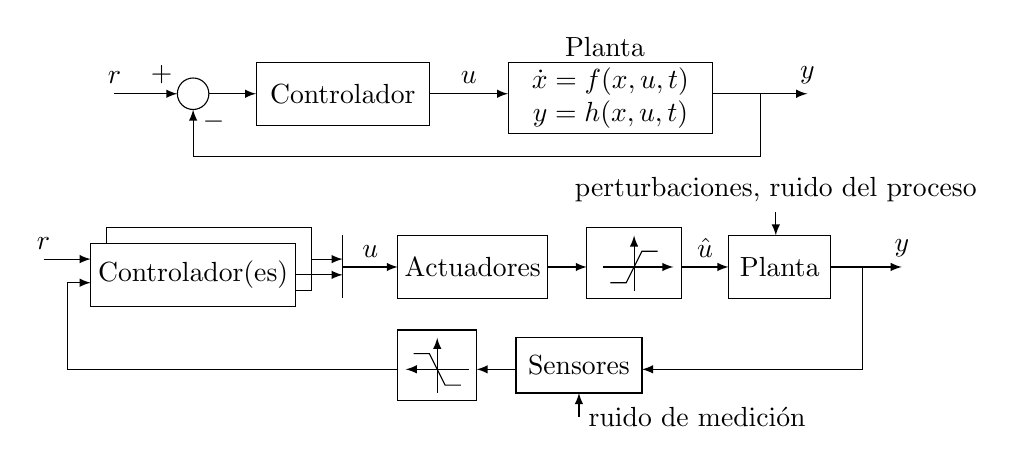
\begin{tikzpicture}
\draw (2.2,4.4) node[right]{Planta};
\draw  (1.6,4.2) rectangle (4.2,3.3) node[midway,align=center] { $\dot{x}=f(x,u,t)$\\$y=h(x,u,t)$ };
\draw [-latex] (0.6,3.8)  -- (1.6,3.8) node[above,midway]{$u$};
\draw  (-1.6,4.2) rectangle (0.6,3.4) node[midway,align=center] {Controlador};
\draw [-latex](-2.2,3.8) -- (-1.6,3.8);
\draw [-latex](-2.4,3.8) ellipse (0.2 and 0.2);
\draw [-latex](-3.4,3.8) node[above] {$r$} -- (-2.6,3.8) node[above, near end] {$+$};
\draw [-latex](4.2,3.8) -- (5.4,3.8) node[above] {$y$};
\draw [-latex](4.8,3.8) -- (4.8,3) -- (-2.4,3) -- (-2.4,3.6) node[right, near end] {$-$};


\draw  (4.4,2) rectangle (5.7,1.2) node[midway,align=center] {Planta};
\draw  (-3.7,1.9) rectangle (-1.1,1.1) node[midway,align=center] {Controlador(es)};
\draw  (2.6,2.1) rectangle (3.8,1.2);
\draw (2.9,1.4)  -- (3.1,1.4) -- (3.3,1.8) -- (3.5,1.8);
\draw [-latex](3.2,1.3) -- (3.2,2);
\draw [-latex](2.8,1.6) -- (3.7,1.6) ;
\draw (-3.5,1.9) -- (-3.5,2.1) -- (-0.9,2.1) -- (-0.9,1.3) -- (-1.1,1.3);
\draw [-latex](3.8,1.6) -- (4.4,1.6) node[above, midway]{$\hat{u}$};
\draw  (0.2,2) rectangle (2.1,1.2) node[midway,align=center] {Actuadores};
\draw [-latex](2.1,1.6) -- (2.6,1.6);
\draw [-latex](-1.1,1.5) -- (-0.5,1.5);
\draw [-latex](-0.9,1.7) -- (-0.5,1.7);
\draw (-0.5,2) -- (-0.5,1.2);
\draw [-latex](-0.5,1.6) -- (0.2,1.6) node[midway, above]{$u$};
\draw [-latex](-4.3,1.7) node[above] {$r$} -- (-3.7,1.7);
\draw  (1.7,0.7) rectangle (3.3,0) node[midway,align=center] {Sensores};
\draw [-latex](5.7,1.6) -- (6.6,1.6) node[above]{$y$};
\draw [-latex](6.1,1.6) -- (6.1,0.3) -- (3.3,0.3);
\draw [-latex](0.2,0.3) -- (-4,0.3) -- (-4,1.4) -- (-3.7,1.4);

\draw [-latex](1.1,0.3) -- (0.3,0.3);
\draw [-latex](0.7,0) -- (0.7,0.7);
\draw (1,0.1) -- (0.8,0.1) -- (0.6,0.5) -- (0.4,0.5);
\draw  (0.2,0.8) rectangle (1.2,-0.1);
\draw [-latex](1.7,0.3) -- (1.2,0.3);
\draw [-latex](2.5,-0.3) node[right]{ruido de medición} -- (2.5,0);
\draw [-latex](5,2.3) node[above]{perturbaciones, ruido del proceso}-- (5,2);

\end{tikzpicture}
		\end{adjustbox}		
	\end{figure}
	
	Objetivo de control: proporcionar $u$, tal que:
	\Activate
	\begin{easylist}[itemize] \ListProperties(Space1=0cm,Space1*=0cm,Space2=0cm,Space2*=0cm)
		& Seguidor: siga a la referencia $r$ (\textit{tracking}).
		& Regulador: regule los estados $x\rightarrow 0$. 
		& En seguidor/regulador rechace perturbaciones: salida/entrada.
	\end{easylist}	
	mientras,
	\Activate
	\begin{easylist}[itemize] \ListProperties(Space1=0cm,Space1*=0cm,Space2=0cm,Space2*=0cm)
		& Cumplir los requerimientos de diseño: \textit{overshoot, settling time}, etc.	
		& Minimizar no linealidades/discontinuidades: \textit{backlash}, relay con histéresis, zona muerta, etc.
		& Minimizar: ruido proceso/medición, error de calibración, error en el modelo de la planta, retraso de tiempo.	
		& \textbf{Satisfacer restricciones físicas (\textit{hard constraints}): max/min torque, voltaje, etc.}
	\end{easylist}
	\Deactivate
\end{frame}

\begin{frame}[fragile]{Con restricciones vs sin restricciones}
	\begin{figure}[!ht]
		\centering
		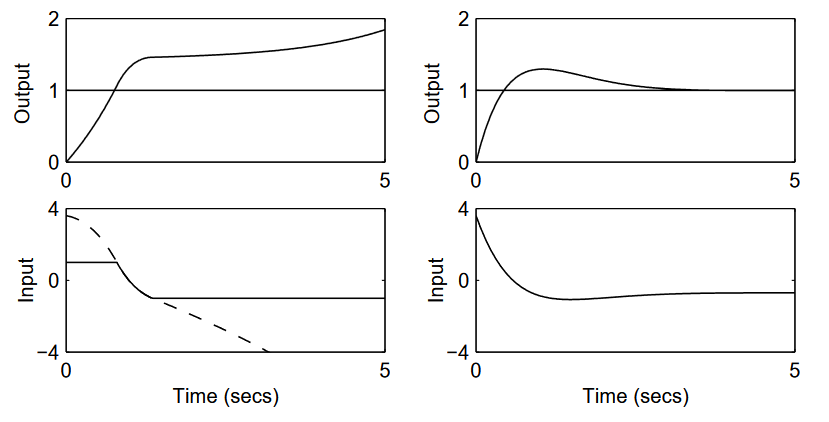
\includegraphics[width=0.7\linewidth]{figures/Contrained_Unconstrained}
		\caption*{Con saturación vs sin saturación - controlador PI}
	\end{figure}	
	Problemas con la saturación: 
	\Activate
	\begin{easylist}[itemize] \ListProperties(Space1=0cm,Space1*=0cm,Space2=0cm,Space2*=0cm)
		& Genera discordancia entre la salida del controlador $u$ y la entrada al sistema $\hat{u}$.
		& Cambios en el controlador no afecta a la planta.
		& Puede permanecer saturado y llevar el sistema a la región de inestabilidad.	
	\end{easylist}
	\Deactivate
	
\end{frame}

\begin{frame}[fragile]{Clásico PID con \textit{anti-windup}\superfullcite{bak2000control}}
	Objetivo: reducir que de la integración del error se dispare (\textit{windup}).
	
	Solución: agregar \textit{feeback loop} de $\Delta(\hat{u}-u)$ con ganancia ajustable $\frac{1}{\tau_i}$ y reset al integrador con una ganancia $\frac{1}{\tau_t}$.
	\begin{figure}[!ht]
		\centering
		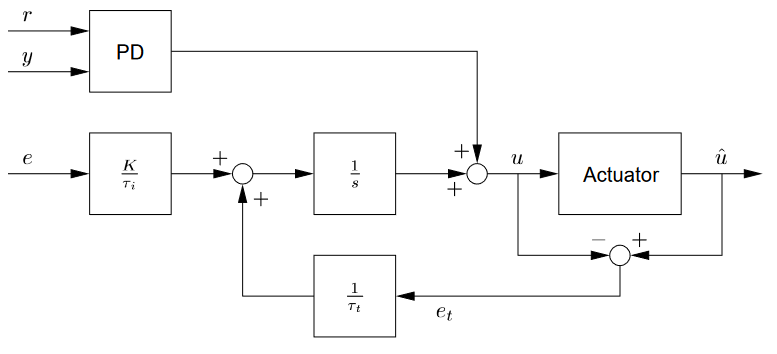
\includegraphics[width=0.7\linewidth]{figures/PID_anti-windup}
		\caption*{PID con anti-windup}
	\end{figure}
	
\end{frame}

\begin{frame}[fragile]{Clásico PID con \textit{anti-windup}}
	Definido como, 
	\begin{equation*}
	\begin{aligned}
	u &= K \left(  e+\frac{1}{\tau_i}\int_{\tau=0}^{t}e(\tau)d\tau+\frac{\tau_i}{K \tau_t}(\hat{u}-u)dt  \right)\\
	\hat{u} &= sat(u)\\
	\end{aligned}		
	\end{equation*}
	en tiempo discreto,
	\begin{equation*}
	\begin{aligned}
	P(k) &= K(\beta r(k)-y(k))\\
	D(k) &= \frac{\alpha \tau_d}{\alpha \tau_d + T}D(k-1) - \frac{K \tau_d}{\alpha \tau_d + T}(1-q^{-1})y(k)\\
	I(k+1) &= I(k) + \frac{K T}{\tau_i} e(k) + \frac{T}{\tau_t} (\hat{u}(k) - u(k))\\
	u(k) &= P(k) + I(k) + D(k)\\
	\hat{u}(k) &= sat(u(k))
	\end{aligned}		
	\end{equation*}
	donde, $\tau_i, \tau_d, \tau_t, \alpha$ y $\beta$ son los parámetros de ajuste.
	
	Pros:
	\Activate
	\begin{easylist}[itemize] \ListProperties(Space1=0cm,Space1*=0cm,Space2=0cm,Space2*=0cm)
		& Implementación fácil.
		& Procesamiento computacional bajo.	
	\end{easylist}
	\Deactivate
	Cons: 
	\Activate
	\begin{easylist}[itemize] \ListProperties(Space1=0cm,Space1*=0cm,Space2=0cm,Space2*=0cm)
		& Ajuste de parámetros por prueba y error.
		& \textbf{No es óptimo}.	
		& \textbf{Manejo de restricciones es a posteriori}.
	\end{easylist}
	\Deactivate
\end{frame}

\begin{frame}[fragile]{LQG (Linear Quadratic Gaussian)}
	Sea un sistema DLTI en espacio de estados,
	\begin{equation}
	\begin{aligned}
		x(k+1) & = A~x(k)+B~u(k)+w(k)               \\
		y(k)   & = C~x(k)+z(k), \quad k=0,1,2,\dots
	\end{aligned}
	\end{equation}
	donde, $x\in\mathbb{R}^n$, $u\in\mathbb{R}^m$, $y\in\mathbb{R}^p$, $w\sim\mathcal{N}(0,Q_w)$, $z\sim\mathcal{N}(0,Q_z)$. Analizando la dinámica,
	\begin{equation*}
	\begin{aligned}
		\dot{x}(k) & = A x(k) + B u(k),      & \dot{\hat{x}}(k)   & = A \hat{x}(k) + B u(k) + L_{KF} (y(k)-\hat{y}(k)) &  \\
		y(k)       & = C x(k),               & \hat{y}(k)         & = C \hat{x}(k)                                     &  \\
		u(k)       & = -K_\infty \hat{x}(k), & \dot{\tilde{x}}(k) & = \dot{x}(k)-\dot{\hat{x}}(k)                      &
	\end{aligned}
	\end{equation*}
	de la dinámica a lazo cerrado, la matriz dinámica es triangular\footnote{$k_r$ reduce el steady-state error (DC gain)}.
	\begin{equation*}
		\begin{bmatrix}
			\dot{x}(k)         \\
			\dot{\tilde{x}}(k)
		\end{bmatrix}
		=
		\begin{bmatrix}
			A-B K_\infty & B K_\infty \\
			0            & A-L_{KF} C
		\end{bmatrix}
		\begin{bmatrix}
			x(k)       \\
			\tilde{x}(k)
		\end{bmatrix}
		+
		\begin{bmatrix}
			B k_r \\
			0
		\end{bmatrix}
		r
	\end{equation*}
	por tanto, el polinomio característico es $\lambda(s) = det(sI-A+B K_\infty)\, det(sI-A+L_{KF} C)$	
	\begin{figure}[!ht]
		\centering
		\begin{adjustbox}{max totalsize={1\textwidth}{1\textheight},center}
			\usetikzlibrary{arrows}
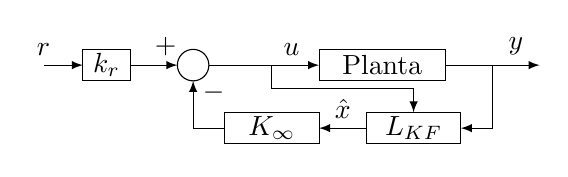
\begin{tikzpicture}
\draw  (1.8,4) rectangle (3.4,3.6) node[midway, align=center] {Planta};
\draw [-latex] (0.4,3.8)  -- (1.8,3.8) node[above, near end]{$u$};
\draw  (0.6,3.2) rectangle (1.8,2.8) node[midway, align=center] {$K_\infty$};

\draw [-latex](0.2,3.8) ellipse (0.2 and 0.2);
\draw [-latex](-0.6,3.8)  -- (0,3.8) node[above, near end] {$+$};
\draw [-latex](3.4,3.8) -- (4.6,3.8) node[above, near end] {$y$};
\draw [-latex](0.6,3) -- (0.2,3) -- (0.2,3.6) node[right, near end] {$-$};

\draw  (2.4,3.2) rectangle (3.6,2.8) node[midway, align=center] {$L_{KF}$};
\draw [-latex](2.4,3) -- (1.8,3) node[above, midway]{$\hat{x}$};
\draw [-latex](4,3.8) -- (4,3) -- (3.6,3);
\draw [-latex](1.2,3.8) -- (1.2,3.5) -- (3,3.5) -- (3,3.2);
\draw  (-1.2,4) rectangle (-0.6,3.6) node[midway, align=center] {$k_r$};
\draw [-latex](-1.7,3.8) node[above] {$r$} -- (-1.2,3.8);
\end{tikzpicture}
		\end{adjustbox}		
	\end{figure}
	\textbf{Principio de separación}: se puede diseñar $K_\infty$ y $L_{KF}$ por separado y luego combinarlos.
	
\end{frame}

\section{LQG vs MPC}
\begin{frame}[fragile]{¿LQG en la industria?}
	\Activate
	\begin{easylist}[itemize] \ListProperties(Space1=0cm,Space1*=0cm,Space2=0cm,Space2*=0cm)
		& Avances teóricos en los 50. (Bellman, Pontryagin, Kalman)
		& Kalman introduce las nociones de controlabilidad y observabilidad.
		& LQR es desarrollado.
		& En 1960 introduce su celebrado filtro\superfullcite{Kalman1960}.
		& Teoría de control óptimo general.
	\end{easylist}
	\Deactivate
	Pero en 1978 \superfullcite{Doyle1978}...
	\begin{figure}[!ht]
		\centering
		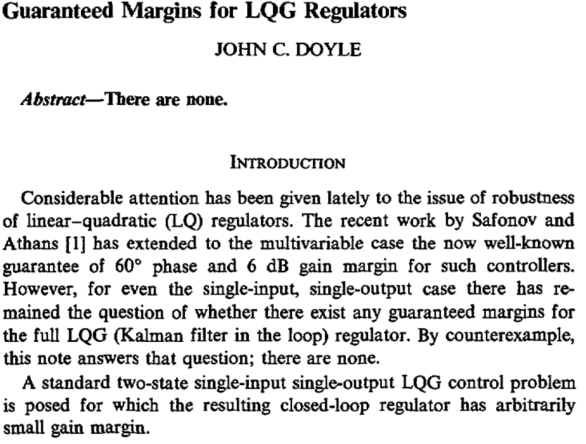
\includegraphics[width=0.65\linewidth]{figures/LQG_Doyle}	
	\end{figure}
\end{frame}

\begin{frame}[fragile]{Raíces del MPC}
	
	\Activate
	\begin{easylist}[itemize] \ListProperties(Space1=0cm,Space1*=0cm,Space2=0cm,Space2*=0cm)
		& Predictor de Smith. (Smith 1970).
		& Control variante mínimo. (Astrom, 1970).
		& Dynamic Matrix Control (DMC). (Cutler y Ramaker, 1980)
	\end{easylist}
	\Deactivate
	
	Gracias al paper seminal de Doyle,
	\Activate
	\begin{easylist}[itemize] \ListProperties(Space1=0cm,Space1*=0cm,Space2=0cm,Space2*=0cm)
		& GPC, MBPC, DMC, RHC,...	
	\end{easylist}
	\Deactivate
	\begin{figure}[!ht]
		\centering
		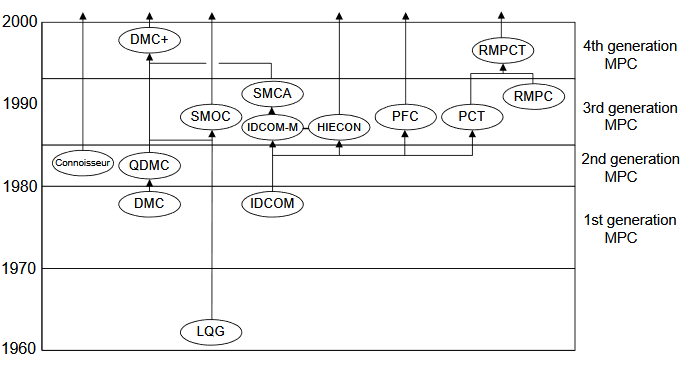
\includegraphics[width=0.8\linewidth]{figures/MPC_genealogy}	
	\end{figure}
\end{frame}

\begin{frame}[fragile]{Unificados finalmente\superfullcite{Mayne2000}}
	
	\begin{figure}[!ht]
		\centering
		
\includegraphics[width=0.65\linewidth]{figures/MPC_Rawlings_Mayne_2000}	
	\end{figure}	
	\textit{"MPC es una técnica donde la acción de control es obtenida resolviendo un problema control óptimo (optimización) a lazo abierto con horizonte finito  de forma on-line para cada instante de tiempo, usando el estado actual como estado inicial. De la secuencia de la solución solo se aplica el primer resultado a la planta y el resto se descarta, cerrando así el lazo. ($H_2$ y $H_\infty$ requieren un horizonte infinito.)"}
	
	\begin{figure}[!ht]
		\centering
		\begin{adjustbox}{max totalsize={.75\textwidth}{1\textheight},center}
			\usetikzlibrary{arrows}
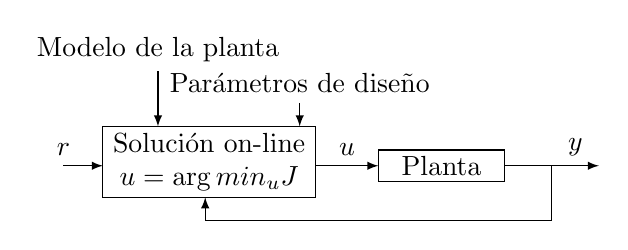
\begin{tikzpicture}
\draw  (1.8,4) rectangle (3.4,3.6) node[midway, align=center] {Planta};





\draw [-latex](3.4,3.8) -- (4.6,3.8) node[above, near end] {$y$};




\draw [-latex](4,3.8) -- (4,3.1) -- (-0.4,3.1)-- (-0.4,3.4);


\draw [-latex](-2.2,3.8) node[above] {$r$} -- (-1.7,3.8);
\draw  (-1.7,4.3) rectangle (1,3.4) node[midway, align=center] {Solución on-line\\$u=\arg min_u J$};
\draw [-latex](1,3.8) -- (1.8,3.8) node[above, midway]{$u$};
\draw [-latex](-1,5) node[above]{Modelo de la planta} -- (-1,4.3);
\draw [-latex](0.8,4.6) node[above]{Parámetros de diseño}  -- (0.8,4.3);
\end{tikzpicture}
		\end{adjustbox}	
	\end{figure}
	
\end{frame}

\section{MPC - idea básica}
\begin{frame}[fragile]{MPC - idea básica}
	\begin{figure}[!ht]
		\centering
		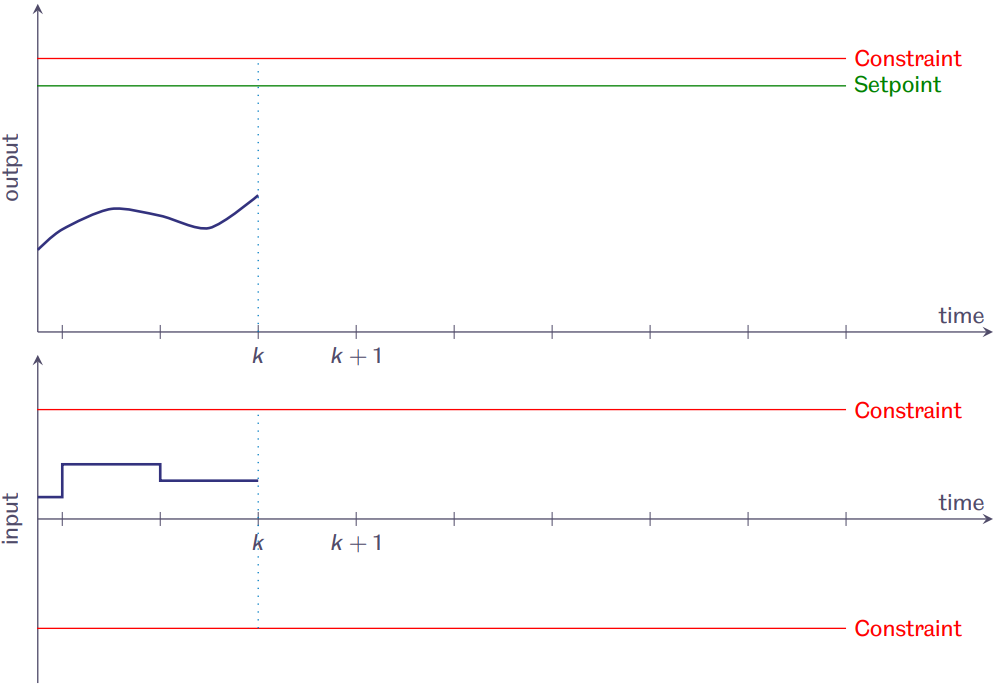
\includegraphics[width=1\linewidth]{figures/MPC_basic_1}	
	\end{figure}
\end{frame}
\begin{frame}[fragile]{MPC - idea básica}
	\begin{figure}[!ht]
		\centering
		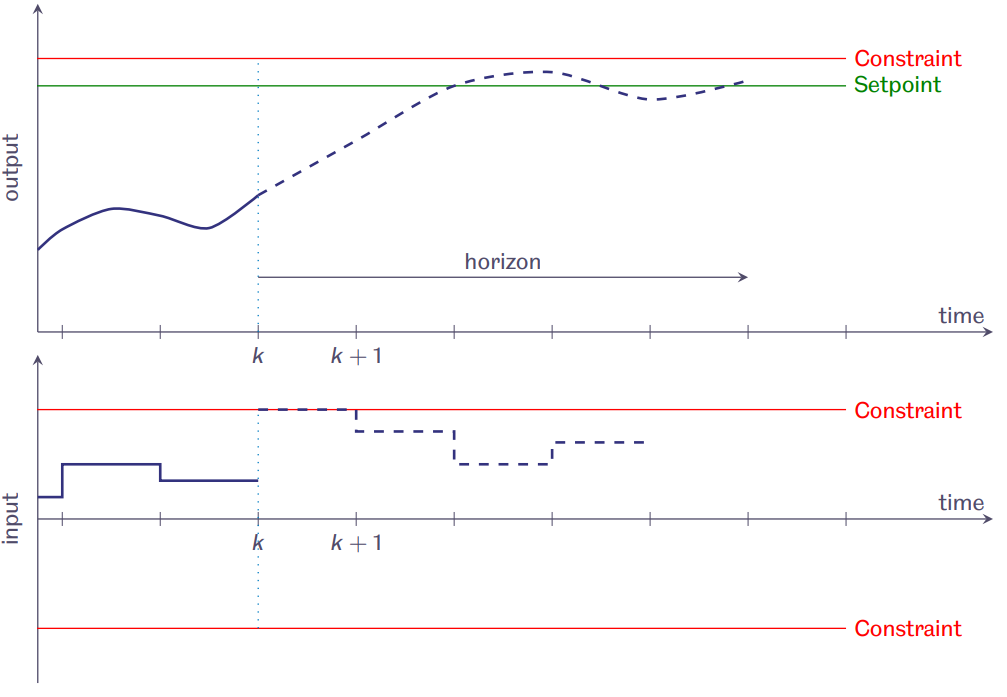
\includegraphics[width=1\linewidth]{figures/MPC_basic_2}	
	\end{figure}
\end{frame}
\begin{frame}[fragile]{MPC - idea básica}
	\begin{figure}[!ht]
		\centering
		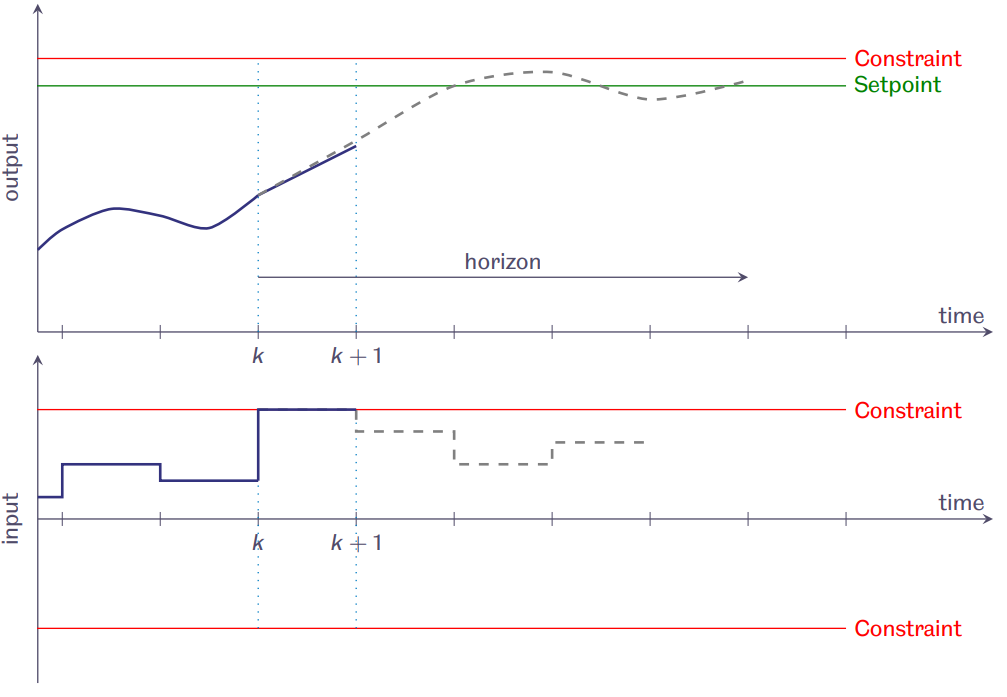
\includegraphics[width=1\linewidth]{figures/MPC_basic_3}	
	\end{figure}
\end{frame}
\begin{frame}[fragile]{MPC - idea básica}
	\begin{figure}[!ht]
		\centering
		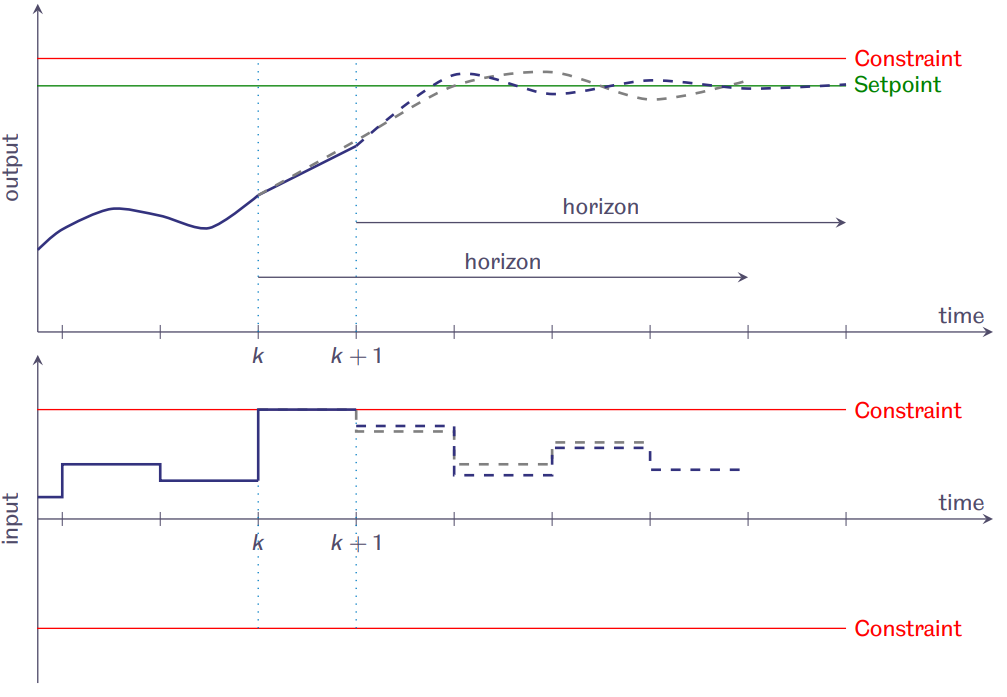
\includegraphics[width=1\linewidth]{figures/MPC_basic_4}	
	\end{figure}
\end{frame}

\section{MPC algoritmo}
\begin{frame}[fragile]{MPC algoritmo}
	\Activate
	\begin{easylist}[itemize] \ListProperties(Space1=0cm,Space1*=0cm,Space2=0cm,Space2*=0cm)
		& Predicción.
		& Optimización.
		& Horizonte reciente. 	
	\end{easylist}
	\Deactivate
\end{frame}


\begin{frame}[fragile]{MPC algoritmo - Predicción}
	\Activate
	\begin{easylist}[itemize] \ListProperties(Space1=0cm,Space1*=0cm,Space2=0cm,Space2*=0cm)
		& Usamos el modelo dinámico de la planta
		& En DTLI,
	\end{easylist}
	\Deactivate
	\begin{equation*}
	\begin{aligned}
		x(k+1) & = f(x(k),u(k)) \\
		y(k)   & = g(x(k))
	\end{aligned}
	\end{equation*}
	\Activate
	\begin{easylist}[itemize] \ListProperties(Space1=0cm,Space1*=0cm,Space2=0cm,Space2*=0cm)
		& Set de predicciones \textbf{futuras} a partir del estado actual para $k$, 	
	\end{easylist}
	\Deactivate
	\begin{equation*}
	\begin{aligned}
		\{u(k|k),u(k+1|k),\dots,u(k+N-1|k)\} \\
		\{x(k|k),x(k+1|k),\dots,x(k+N|k)\}\\
		\{y(k|k),y(k+1|k),\dots,y(k+N|k)\}
	\end{aligned}
	\end{equation*}
\end{frame}



\begin{frame}[fragile]{MPC algoritmo - Optimización}
	\Activate
	\begin{easylist}[itemize] \ListProperties(Space1=0cm,Space1*=0cm,Space2=0cm,Space2*=0cm)
		& A partir de ese set, minimizar una función de costo,
	\end{easylist}
	\Deactivate
	\begin{equation*}
		J_N = \sum_{j=0}^{N-1} \mathcal{L}( x(k+j|k), u(k+j|k) )
	\end{equation*}
	mientras satisfaga cualquier restricción en,
	\begin{equation*}
	\begin{aligned}
		u_{min}\leq u(k) \leq u_{max}\\
		x_{min}\leq x(k) \leq x_{max}\\
		y_{min}\leq y(k) \leq y_{max}\\
	\end{aligned}
	\end{equation*}
	
\end{frame}

\begin{frame}[fragile]{MPC algoritmo - Horizonte de retroceso (reciente)}

	\Activate
	\begin{easylist}[itemize] \ListProperties(Space1=0cm,Space1*=0cm,Space2=0cm,Space2*=0cm)
		& Aplicando solo el primer resultado de la solución al problema de optimización,
	\end{easylist}
	\Deactivate
	\begin{equation*}
	\begin{aligned}
		\mathbf{u}^*(k) & = \mathrm{arg}\min_{u(k)}~ J_N      \\
              			& = \left\{ { \color{red} u^*(k|k) } ,u^*(k+1|k),\dots,u^*(k+N-1|k) \right\}
	\end{aligned}
	\end{equation*}
	\Activate
	\begin{easylist}[itemize] \ListProperties(Space1=0cm,Space1*=0cm,Space2=0cm,Space2*=0cm)
		& Se cierra el lazo y la planta cambia,	
	\end{easylist}
	\Deactivate
	\begin{equation*}
	\begin{aligned}
		x(k+1) & = \tilde{f}(x(k),{ \color{red} u^*(k) }) \\
		y(k+1) & = \tilde{g}(x(k))
	\end{aligned}
	\end{equation*}
	\Activate
	\begin{easylist}[itemize] \ListProperties(Space1=0cm,Space1*=0cm,Space2=0cm,Space2*=0cm)
		& Se repite el proceso para el siguiente instante de tiempo $k+1$.	
	\end{easylist}
	\Deactivate
\end{frame}

\begin{frame}[fragile]{MPC algoritmo}
	\begin{figure}[!ht]
		\centering
		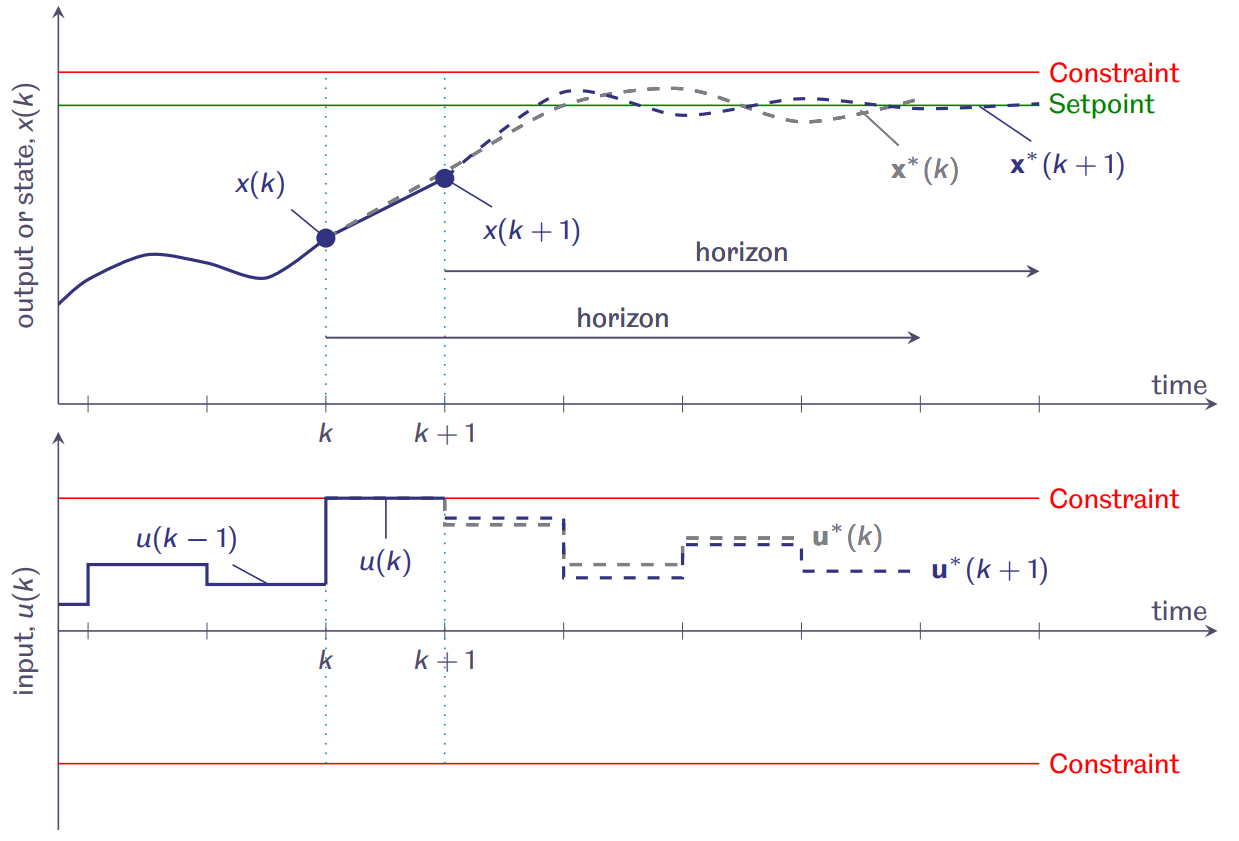
\includegraphics[width=1\linewidth]{figures/MPC_basic_4a}	
	\end{figure}
\end{frame}


\begin{frame}[fragile]{MPC es una familia de algoritmos}
	Los sistemas pueden ser,
	\Activate
	\begin{easylist}[itemize] \ListProperties(Space1=0cm,Space1*=0cm,Space2=0cm,Space2*=0cm)
		& Lineales o no lineales.
		& Continuos o discretos.
		& Híbridos (continuo+discreto).  
		& Deterministico o estocástico.	
	\end{easylist}
	\Deactivate
	
	y se necesita como prerequisito,
	\Activate
	\begin{easylist}[itemize] \ListProperties(Space1=0cm,Space1*=0cm,Space2=0cm,Space2*=0cm)
		& Teoría de espacio de estados.		
		& Control óptimo (LQR).
		& Optimización convexa (funciones cuadrática). \textbf{Importante!}
		& Programación dinámica (optimización multi-etapa).	
		& Sistemas no lineales (estabilidad de Lyapunov).
		& ...
	\end{easylist}
	\Deactivate
\end{frame}

\section{Control por MPC}
\begin{frame}[fragile]{Control por MPC}	
	Sea un sistema DLTI en espacio de estados,
	\begin{equation}
	\begin{aligned}
	x(k+1) & = A~x(k)+B~u(k)+w(k)               \\
	y(k)   & = C~x(k)+z(k), \quad k=0,1,2,\dots
	\end{aligned}
	\end{equation}
	donde $x\in\mathbb{R}^n$, $u\in\mathbb{R}^m$, $y\in\mathbb{R}^p$, $w\sim\mathcal{N}(0,Q_w)$, $z\sim\mathcal{N}(0,Q_z)$. 
	
	El objetivo de control es regular $x\rightarrow 0$ mientras se minimize la función de costo,
	\begin{align}
		J_N & = \sum_{j=0}^{N-1} \mathcal{L}( x(k+j|k), u(k+j|k) )          \nonumber                                                       \\
		J_N & = \sum_{j=0}^{N-1} \left( \|x(k+j|k)\|^2_Q + \|u(k+j|k)\|^2_R \right) + \|x(k+N|k)\|^2_P     \label{eq:MPC}                   \\
		J_N & = \sum_{j=0}^{N-1} (x^\intercal(k+j|k)~Q~x(k+j|k)+ u^\intercal(k+j|k)~R~u(k+j|k) )  + x^\intercal(k+N|k)~P~x(k+N|k) \nonumber
	\end{align}
	\qquad sujeto a, 
	\begin{align*}
		x(k+1+j|k)                   & = A~x(k+j|k)+B~u(k+j|k)  \\
		x(k|k)                       & = x(k)                   \\
		\color{blue}P_x~x(k+j|k)     & \color{blue}\leq q_x     \\
		\color{blue}P_u~u(k+j|k)     & \color{blue}\leq q_u     \\
		\color{blue}P_{x_N}~x(k+N|k) & \color{blue}\leq q_{x_N}
	\end{align*}
	\qquad para $ j=0,1,2,\dots,N-1$, y $k=0,1,2,\dots$\\
	
	Donde $Q\succeq 0$, $P\succeq 0$, $R\succ 0$, y $Q\in\mathbb{R}^{n\times n}$, $P\in\mathbb{R}^{n\times n}$, $R\in\mathbb{R}^{m\times m}$ y $N \in\mathbb{N}$. $P_x x\leq q_x$, $P_u u\leq q_u$, y $P_{x_N} x\leq q_{x_N}$ son las restricciones (polihedros). 
	
\end{frame}

\begin{frame}[fragile]{Matriz de predicción de la dinámica del sistema}	
	Recurvisamente,
	\begin{align*}
	x(k+1|k) &= A~x(k)+B~u(k) \\
	x(k+2|k) &= A~x(k+1|k)+B~u(k+1|k) \\
	&= A^2~x(k)+AB~u(k|k)+B~u(k+1|k) \\
	\vdots \hspace{2em}  &= \hspace{3em} \vdots \\
	x(k+N|k) &= A~x(k+N-1|k)+B~u(k+N-1|k) \\
	&= A^N~x(k)+A^{N-1}B~u(k|k)+\dots+B~u(k+N-1|k)
	\end{align*}
	agrupando,
	\begin{equation}
	\begin{aligned}
	{\underbrace{
			\begin{bmatrix}
			x(k+1|k) \\
			x(k+2|k) \\
			\vdots \\
			x(k+N|k)
			\end{bmatrix}}_{\mathbf{x}(k)}
	}
	=
	{\underbrace{
			\begin{bmatrix}
			A \\
			A^2 \\
			\vdots \\
			A^N
			\end{bmatrix}}_{F}
	}
	+
	{\underbrace{
			\begin{bmatrix}
			B        & 0        & \dots  & 0      \\
			AB       & B        & \dots  & 0      \\
			\vdots   & \vdots   & \ddots & \vdots \\
			A^{N-1}B & A^{N-2}B & \dots  & B
			\end{bmatrix}}_{G}
	}
	{\underbrace{
			\begin{bmatrix}
			u(k|k) \\
			u(k+1|k) \\
			\vdots \\
			u(k+N-1|k)
			\end{bmatrix}}_{\mathbf{u}(k)}
	}
	\end{aligned}
	\end{equation}
	la predicción de la dinámica resulta en,
	\begin{equation}\label{eq:PredictionEqConstraint}
	\mathbf{x}(k) = F~x(k)+G~\mathbf{u}(k)
	\end{equation}
	donde $\mathbf{x}(k)$, y $\mathbf{u}(k)$ son los vectores de estados y entradas predecidas para $j=0,1,2,\dots,N$.
\end{frame}


\begin{frame}[fragile]{Matriz de predicción de la función de costo}	
	Reescribiendo la función de costo \eqref{eq:MPC} como,
	\begin{equation}
	\begin{aligned}
	x^\intercal(k|k)~Q~x(k|k)
	&+
	\begin{bmatrix}
		x(k+1|k) \\
		x(k+2|k) \\
		\vdots   \\
		x(k+N|k)
	\end{bmatrix}^\intercal
	{\underbrace{
			\begin{bmatrix}
				Q      & 0      & \dots  & 0      \\
				0      & Q      & \ddots & \vdots \\
				\vdots & \ddots & Q      & 0      \\
				0      & \dots  & 0      & P
			\end{bmatrix}}_{\tilde{Q}}
	}
	\begin{bmatrix}
		x(k+1|k) \\
		x(k+2|k) \\
		\vdots   \\
		x(k+N|k)
	\end{bmatrix}
	\\
	&+
	\begin{bmatrix}
		u(k|k)     \\
		u(k+1|k)   \\
		\vdots     \\
		u(k+N-1|k)
	\end{bmatrix}^\intercal
	{\underbrace{
			\begin{bmatrix}
				R      & 0      & \dots  & 0      \\
				0      & R      & \ddots & \vdots \\
				\vdots & \ddots & R      & 0      \\
				0      & \dots  & 0      & R
			\end{bmatrix}}_{\tilde{R}}
	}
	\begin{bmatrix}
		u(k|k)     \\
		u(k+1|k)   \\
		\vdots     \\
		u(k+N-1|k)
	\end{bmatrix}
	\end{aligned}
	\end{equation}
	
	Ahora, con $x(k|k)=x(k)$, el problema es minimizar,
	\begin{equation}\label{eq:PredictionCost}
	J_N(x(k),\mathbf{u}(k)) =  x^\intercal(k)~Q~x(k) + \mathbf{x}^\intercal(k)~\tilde{Q}~\mathbf{x}(k) + \mathbf{u}^\intercal(k)~\tilde{R}~\mathbf{u}(k) 
	\end{equation}
	\qquad sujeto a,
	\begin{equation*}
	\mathbf{x}(k) = F~x(k)+G~\mathbf{u}(k)
	\end{equation*}
\end{frame}


\begin{frame}[fragile]{Matriz de predicción de la función de costo}	

	Entonces sustituyendo \eqref{eq:PredictionEqConstraint} en \eqref{eq:PredictionCost},
	\begin{equation*}
		J_N(x(k),\mathbf{u}(k)) =  x^\intercal(k) Q x(k) + ( F x(k)+G \mathbf{u}(k) )^\intercal \tilde{Q} ( F x(k)+G \mathbf{u}(k) ) + \mathbf{u}^\intercal(k)~\tilde{R} \mathbf{u}(k)
	\end{equation*}
	y realizando operaciones algebraicas, la función de costo en su forma compacta QP \footnote{QP unconstrained} es,
	\begin{align}
		J_N(x(k),\mathbf{u}(k)) = \frac{1}{2} \mathbf{u}(k)^\intercal~H~\mathbf{u}(k)+c^\intercal~\mathbf{u}(k)+\alpha
	\end{align}
	donde, 
	\begin{equation}
	\begin{aligned}
		H      & =2(G^\intercal\tilde{Q}G+\tilde{R}) \\
		c      & =L~x(k)                             \\
		L      & = 2G^\intercal\tilde{Q}F            \\
		\alpha & =x^\intercal(k)~M~x(k)              \\
		M      & =Q+F^\intercal\tilde{Q}F
	\end{aligned}
	\end{equation}

\end{frame}

\section{Polihedros}
\begin{frame}[fragile]{Polihedros - inecuaciones lineales}
	Si, $x=\begin{bmatrix}
		x_1 \\
		x_2
	\end{bmatrix}$ y $u$ es escalar. Las restriciones (saturación),
	\begin{equation*}
		x_{min} \leq x(k+j|k) \leq x_{max}, \qquad u_{min} \leq u(k+j|k) \leq u_{max}
	\end{equation*}
	se pueden transforma a inecuaciones como,	
	\begin{align*}
	\begin{bmatrix}
		+1 & 0  \\
		0  & +1 \\
		-1 & 0  \\
		0  & -1
	\end{bmatrix}
	x(k+j|k) & \leq
	\begin{bmatrix}
		+x_{max,1}  \\
		+x_{max,2}  \\
		-x_{min,1}  \\
		-x_{min,2} 
	\end{bmatrix}
	\\
	\begin{bmatrix}
		+1 \\
		-1
	\end{bmatrix}
	u(k+j|k) & \leq
	\begin{bmatrix}
		+u_{max}  \\
		-u_{min}
	\end{bmatrix}
	\end{align*}
\end{frame}

\begin{frame}[fragile]{Polihedros - inecuaciones lineales}
	En general,
	\begin{equation*}
	\begin{aligned}
		{\underbrace{
			\begin{bmatrix}
			+I_{n\times n} \\
			-I_{n\times n}
			\end{bmatrix}}_{P_x}
		}
		x(k+j|k) & \leq
		{\underbrace{
			\begin{bmatrix}
			+x_{max}\\
			-x_{min}
			\end{bmatrix}}_{q_x}
		}
		%
		\\
		{\underbrace{
			\begin{bmatrix}
			+I_{m\times m} \\
			+I_{m\times m}
			\end{bmatrix}}_{P_u}
		}
		u(k+j|k) & \leq
		{\underbrace{
			\begin{bmatrix}
			+u_{max}\\
			-u_{min}
			\end{bmatrix}}_{q_u}
		}
	\end{aligned}
	\end{equation*}
	y para,
	\begin{equation*}
	y_{min} \leq y(k+j|k) \leq y_{max}
	\end{equation*}
	es equivalente a,
	\begin{equation*}
	\begin{aligned}
		{\underbrace{
			\begin{bmatrix}
			+C \\
			-C
			\end{bmatrix}}_{P_x}
		}
		x(k+j|k) & \leq
		{\underbrace{
			\begin{bmatrix}
			+y_{max}\\
			-y_{min}
			\end{bmatrix}}_{q_x}
		}
	\end{aligned}
	\end{equation*}
	
\end{frame}


\begin{frame}[fragile]{Polihedro de predicción de las restricciones (estados)}	
	Definiendo las restricciones de los estados como,
	\begin{align*}
	\begin{cases}
	P_x~x(k+j|k) &\leq q_x\\
	P_{x_N}~x(k+N|k) &\leq q_{x_N}
	\end{cases}
	\end{align*}
	agrupando\footnote{$P_{x_N},~q_{x_N}$ restricciones terminales que definen la estabilidad del sistema.},
	\begin{equation*}
	\begin{aligned}
	\underbrace{
		\begin{bmatrix}
		P_x\\
		0\\
		0\\
		\vdots\\
		0
		\end{bmatrix}
	}_{\tilde{P}_{x_0}}
	x(k|k)
	+
	\underbrace{
		\begin{bmatrix}
			0      & 0      & \dots  & 0                        \\
			P_x    & 0      & \dots  & 0                        \\
			0      & P_x    & \dots  & 0                        \\
			\vdots & \vdots & \ddots & \vdots                   \\
			0      & 0      & \dots  & { \color{blue} P_{x_N} }
		\end{bmatrix}
	}_{\tilde{P}_x}
	\underbrace{
		\begin{bmatrix}
		x(k+1|k)\\
		x(k+2|k)\\
		\vdots\\
		x(k+N|k)
		\end{bmatrix}
	}_{\mathbf{x}(k)}
	\leq
	\underbrace{
		\begin{bmatrix}
		q_x\\
		q_x\\
		q_x\\
		\vdots\\
		q_{x_N}
		\end{bmatrix}
	}_{\tilde{q}_x}
	\end{aligned}
	\end{equation*}
	resulta en,
	\begin{align}\label{eq:Px_tilde}
	\tilde{P}_x~\mathbf{x}(k)\leq \tilde{q}_x - \tilde{P}_{x_0}~x(k)
	\end{align}
	
	
\end{frame}


\begin{frame}[fragile]{Polihedro de predicción de las restricciones (entrada)}
	Las restricciones de entrada son,
	\begin{align*}
	P_u~u(k+j|k)\leq q_u
	\end{align*}
	agrupando,
	\begin{equation*}
	\begin{aligned}
	\underbrace{
		\begin{bmatrix}
			P_u    & 0      & \dots  & 0      \\
			0      & P_u    & \dots  & 0      \\
			\vdots & \vdots & \ddots & \vdots \\
			0      & 0      & \dots  & P_u
		\end{bmatrix}
	}_{\tilde{P}_u}
	\underbrace{
		\begin{bmatrix}
			u(k|k)     \\
			u(k+1|k)   \\
			\vdots     \\
			u(k+N-1|k)
		\end{bmatrix}
	}_{\mathbf{u}(k)}
	\leq
	\underbrace{
		\begin{bmatrix}
			q_u    \\
			q_u    \\
			\vdots \\
			q_u
		\end{bmatrix}
	}_{\tilde{q}_u}
	\end{aligned}
	\end{equation*}
	resulta en,
	\begin{align}
	\tilde{P}_u~\mathbf{u}(k)\leq \tilde{q}_u
	\end{align}
	
\end{frame}


\begin{frame}[fragile]{Agrupando ambos polihedros}
	Agrupando ambos polihedros en forma compacta,
	\begin{align*}
	\begin{cases}
		\tilde{P_u}~\mathbf{u}(k) & \leq \tilde{q_u}                      \\
		\tilde{P_x}~\mathbf{x}(k) & \leq \tilde{q_x}-\tilde{P}_{x_0}~x(k)
	\end{cases}
	\end{align*}
	usando \eqref{eq:PredictionEqConstraint} para eliminar $\mathbf{x}(k)$,
	\begin{align*}
		\tilde{P_x}(F~x(k)+G~\mathbf{u}(k)) & \leq \tilde{q_x}-\tilde{P}_{x_0}~x(k)                  \\
		\tilde{P_x}~G~\mathbf{u}(k)         & \leq \tilde{q_x}+(-\tilde{P}_{x_0}-\tilde{P_x}~F)~x(k)
	\end{align*}
	agrupando,
	\begin{equation}
	\begin{aligned}
		\underbrace{
			\begin{bmatrix}
			\tilde{P_u}\\
			\tilde{P_x}~G
			\end{bmatrix}
		}_{P_c}
		\mathbf{u}(k)
		\leq
		\underbrace{
			\begin{bmatrix}
			\tilde{q_u}\\
			\tilde{q_x}
			\end{bmatrix}
		}_{q_c}
		+
		\underbrace{
			\begin{bmatrix}
			0\\
			-\tilde{P}_{x_0}-\tilde{P_x}~F
			\end{bmatrix}
		}_{S_c}
		x(k)
	\end{aligned}
	\end{equation}
	entonces,
	\begin{align}\label{eq:ConstraintPredicedtMatrices}
	P_c~\mathbf{u}(k) \leq q_c+S_c~x(k)
	\end{align}
		

\end{frame}



\begin{frame}[fragile]{Al fin!...}
	El problema de control MPC con restricciones en su forma compacta es minimizar,
	\begin{align}
	J^*_N(x(k),\mathbf{u}(k)) & = \min_{\mathbf{u}(k)}~\frac{1}{2} \mathbf{u}(k)^\intercal~H~\mathbf{u}(k)+c^\intercal~\mathbf{u}(k)+\alpha
	\intertext{sujeto a,}
	P_c~\mathbf{u}(k) & \leq q_c+S_c~x(k) \nonumber
	\end{align}
	donde la solución óptima es,
	\begin{equation}\label{eq:opt_mpc_c}
	\begin{aligned}
		\mathbf{u}^*(k) &= \mathrm{arg}\min_{u(k)}~	
		\left.
		\begin{cases}
			\dfrac{1}{2} \mathbf{u}(k)^\intercal H \mathbf{u}(k)+x^\intercal(k) L^\intercal \mathbf{u}(k)+\alpha~: P_c \mathbf{u} \leq q_c+S_c x(k)
		\end{cases} 
		\hspace{-1em}\right\}
		\\
		\mathbf{u}^*(k)&= \left\{ {\color{red}u^*(k|k)},u^*(k+1|k),\dots,u^*(k+N-1|k) \right\}
	\end{aligned} 
	\end{equation}	
	
	$u^*(k|k)$ es la ley de control no lineal implícita de tiempo invariante que se aplica a la planta y que considera las restricciones/saturaciones a priori,
	\begin{equation}
		u^*(k|k) = \kappa_N \left( x(k) \right)
	\end{equation}
	que además está listo para introducir a su optimizador favorito, e.g. \texttt{quadprog} en Matlab, \texttt{ACADOS} para sistemas embebidos.\\
	
\end{frame}

\begin{frame}{Los sets}
	La región de viabilidad (\textit{feasibility region})  $\mathcal{X}_N$ es el set de estados para los cuales la función de costo tiene solución,
	\begin{align}
	\mathcal{X}_N = \{x(k):\mathcal{U}_N(x(k)) \neq 0\}
	\end{align}
	donde el set viable $\mathcal{U}_N$ es,
	\begin{align}
	\mathcal{U}_N(x(k)) &= \{ \mathbf{u}(k) : P_c~\mathbf{u}(k) \leq q_c+S_c~x(k) \}
	\intertext{Set de restricciones de entrada,}
	\mathcal{U} &=\{ u(k) : P_u~u(k)\leq q_u \} \subseteq \mathbb{R}^m\\
	\intertext{set de restricciones de estados,}
	\mathcal{X} &=\{ x(k) : P_x~x(k)\leq q_x \} \subseteq \mathbb{R}^n\\
	\intertext{y el set de restricciones terminal,}
	\mathcal{X}_f &=\{ x(k) : P_{x_N}~x(k)\leq q_{x_N} \} \subseteq \mathbb{R}^n
	\end{align}
\end{frame}

\section{Estabilidad por Lyapunov}
\begin{frame}[fragile]{Estabilidad por Lyapunov - no lineal}
	Definición,
	\begin{figure}[!ht]
		\centering
		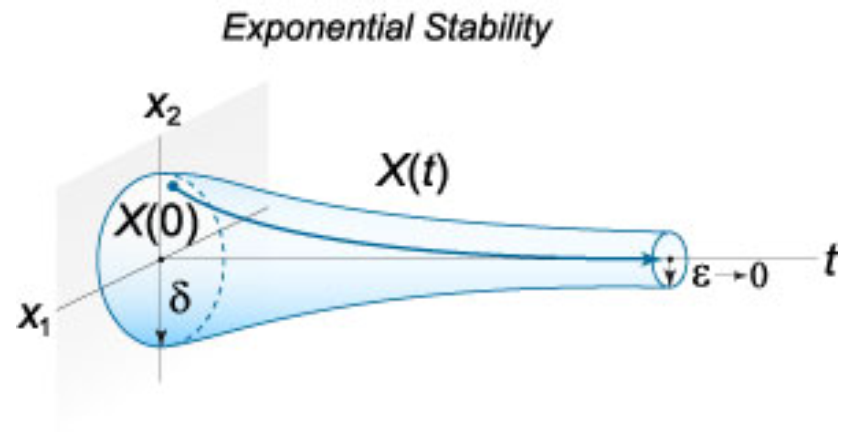
\includegraphics[width=0.6\linewidth]{figures/Lyapunov}	
	\end{figure}
	Para un sistema $x^+=f(x)$, el origen $x=0$ es \textbf{exponencialmente estable} en una región de atracción $\mathcal{X}$ si existe un $c>0$ y un $\gamma\in (0,1)$ tal que,
	\begin{align*}
	|x(k)|\leq c~\gamma^k |x(0)| \text{ para todo } x(0)\in \mathcal{X} \text{ y } k>0
	\end{align*}
	
\end{frame}


\begin{frame}[fragile]{Estabilidad no lineal en MPC}
	Para garantizar estabilidad, el objetivo es construir un set terminal de restricciones $\mathcal{X}_f$ para que exista solución después del horizonte $N$ y satisfaga las restricciones del problema en modo-2,
	\begin{equation}\label{eq:constraints_mode-2}
	\begin{aligned}
		x(k+N+j|k) & \in \mathcal{X},~j=1,2,... \\
		u(k+N+j|k) & \in \mathcal{U},~j=1,2,...
	\end{aligned}  
	\end{equation}
	
	Usando un controlador deadbeat para el modo-2, es decir, $j=N,\dots,N+n-1$, en \eqref{eq:constraints_mode-2},
	\begin{equation}
	\begin{aligned}
		x(k+j|k) & = (A+B~K)^j~x(k+N|k)  \\
		u(k+j|k) & = K(A+B~K)^j~x(k+N|k)
	\end{aligned}
	\end{equation}
	extendiendo las restricciones en $n$ pasos después del modo-1, 
	\begin{equation}
	\begin{aligned}
	\underbrace{
		\overbrace{
			\begin{bmatrix}
			Px    & 0     & \dots & 0     \\
			P_u K & 0     & \dots & 0     \\
			0     & P_x   & \dots & 0     \\
			0     & P_u K & \dots & 0     \\
			\dots & \dots & \dots & \dots
			\end{bmatrix}
		}^{\mathcal{M}}
		\begin{bmatrix}
		(A+B K)^0\\
		(A+B K)^1 \\
		\vdots\\
		(A+B K)^{n-1}
		\end{bmatrix}
	}_{P_{x_N}}
	x(k+N|k)
	\leq
	\underbrace{
		\begin{bmatrix}
		q_x\\
		q_u\\
		q_x\\
		q_u\\
		\vdots
		\end{bmatrix}
	}_{q_{x_N}}
	\end{aligned}
	\end{equation}
	Entonces, para cualquier $x(k+N|k) \in \mathcal{X}_f$ 
	\begin{align}\label{eq:Xf}
	\mathcal{X}_f = \{ x(k+N|k) \in \mathbb{R}^n : P_{x_N}~x(k+N|k) \leq q_{x_N} \}
	\end{align}
	
	$\mathcal{X}_f$ tiene la propiedad de set invariante, lo que significa que las predicciones del sistema en modo-2 se quedarán en $\mathcal{X}_f$ para $k\rightarrow\infty$.
\end{frame}


\begin{frame}{Modo-1 y modo-2}
	\begin{figure}[!ht]
		\centering
		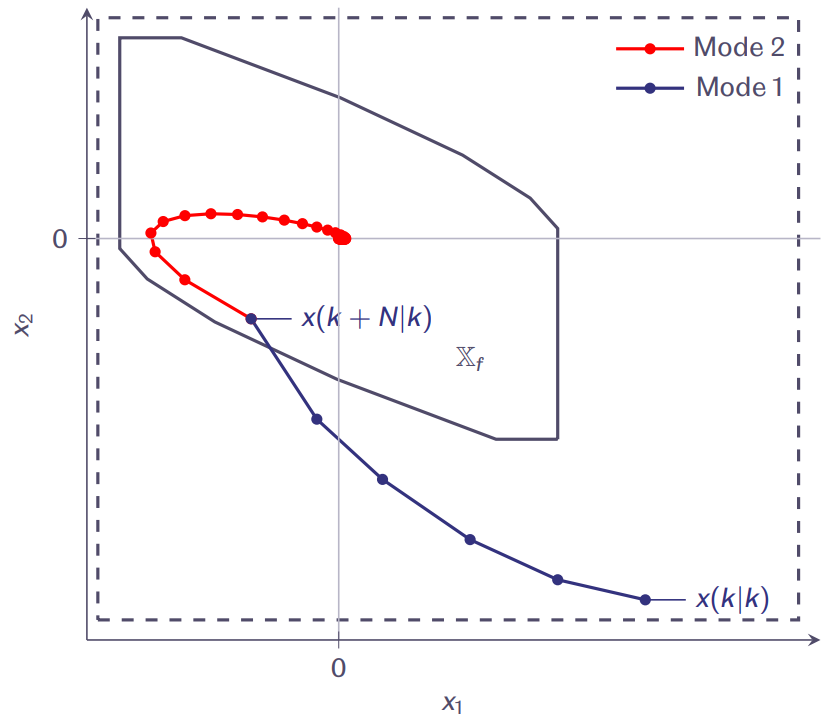
\includegraphics[width=0.7\linewidth]{figures/mode-1_mode-2}
	\end{figure}
\end{frame}

\begin{frame}[fragile]{Estabilidad en MPC}
	En conclusión, la estabilidad es garantizada si,
	\Activate
	\begin{easylist}[itemize] \ListProperties(Space1=0cm,Space1*=0cm,Space2=0cm,Space2*=0cm)
		& $(A,B)$ es estabilizable.
		& $Q\succeq 0,~R\succ 0$
		& $(Q^{1/2},A)$ es observable. ($Q^{1/2}=C$)
		& $P$ satisface la ecuación de Lyapunov para un estabilizador $K$ (LQR),\\
		$(A+B~K)^\intercal~P~(A+B~K)-P=-(Q+K^\intercal~R~K)$
		& $\mathcal{X}_f$ es un set invariante para la dinámica del modo-2: $x(k+1)=(A+B~K)~x(k)$
	\end{easylist}
	\Deactivate
	entonces, dado un $x(k)\in \mathcal{X}_N$,
	\Activate
	\begin{easylist}[itemize] \ListProperties(Space1=0cm,Space1*=0cm,Space2=0cm,Space2*=0cm)
		& $J^*_N(x(k))$ es una función de Lyapunov para la dinámica del modo-1: $x(k+1)=Ax(k)+B\kappa_N(x(k))$, y es recursivamente viable, esto es: si existe una solución viable $J^*_N(x(k))$, entonces las soluciones subsecuentes  ${J^*_N(x(k+1)),~J^*_N(x(k+2)),\dots}$ existen y son viables en  $\mathcal{X}_N$.
		& Todas las restricciones se satisfacen.
		& El origen $x=0$ es asimptoticamente estable en una Región de Atracción (RoA) $\mathcal{X}_N$.
		& $\mathcal{X}_N$ es un set invariante para la dinámica en modo-1: $x(k+1)=Ax(k)+B\kappa_N(x(k))$.
	\end{easylist}
	\Deactivate
	
\end{frame}

\section{Ejemplo MPC}
\begin{frame}[fragile]{Ejemplo MPC}
	Sistema inestable de fase no-mínima,
	\begin{align*}
		x(k+1) 
		&= 
		\begin{bmatrix}
		1.12 & 0.20 \\
		0.11 & 1.01
		\end{bmatrix}
		x(k)+
		\begin{bmatrix}
		0.11\\
		0.06
		\end{bmatrix}
		u(k)+w(k)\\
		y(k) &= 
		\begin{bmatrix}
		-1 & 1
		\end{bmatrix}
		x(k) + z(k)\\
		x(0) & = [0 \quad 1.5]^\intercal\\
		Ts &= 0.1, \quad N = 10, \quad k = 100\\
		Q &= 
		\begin{bmatrix}
		1e^6 & 0 \\
		0 & 1e^6
		\end{bmatrix}
		,\quad R = 1\\
		w(k) & \sim \mathcal{N}(0,0.01), \quad z(k) \sim \mathcal{N}(0,0.01)
	\end{align*}
	Restricciones,
	\begin{align*}
		|x| \leq 2, \quad |u| \leq 10
	\end{align*}
	
%	Ataque DoS,
%	\begin{align*}
%	\nu(k) & \sim \mathcal{B}(0.8), \quad \gamma \sim \mathcal{B}(0.5)
%	\end{align*}
%	Ataque FDI,
%	\begin{align*}
%	c & = [0 \quad 0.2]^\intercal
%	\end{align*}
	
\end{frame}

\begin{frame}{Ejemplo}
	\begin{figure}[!ht]
		\centering
		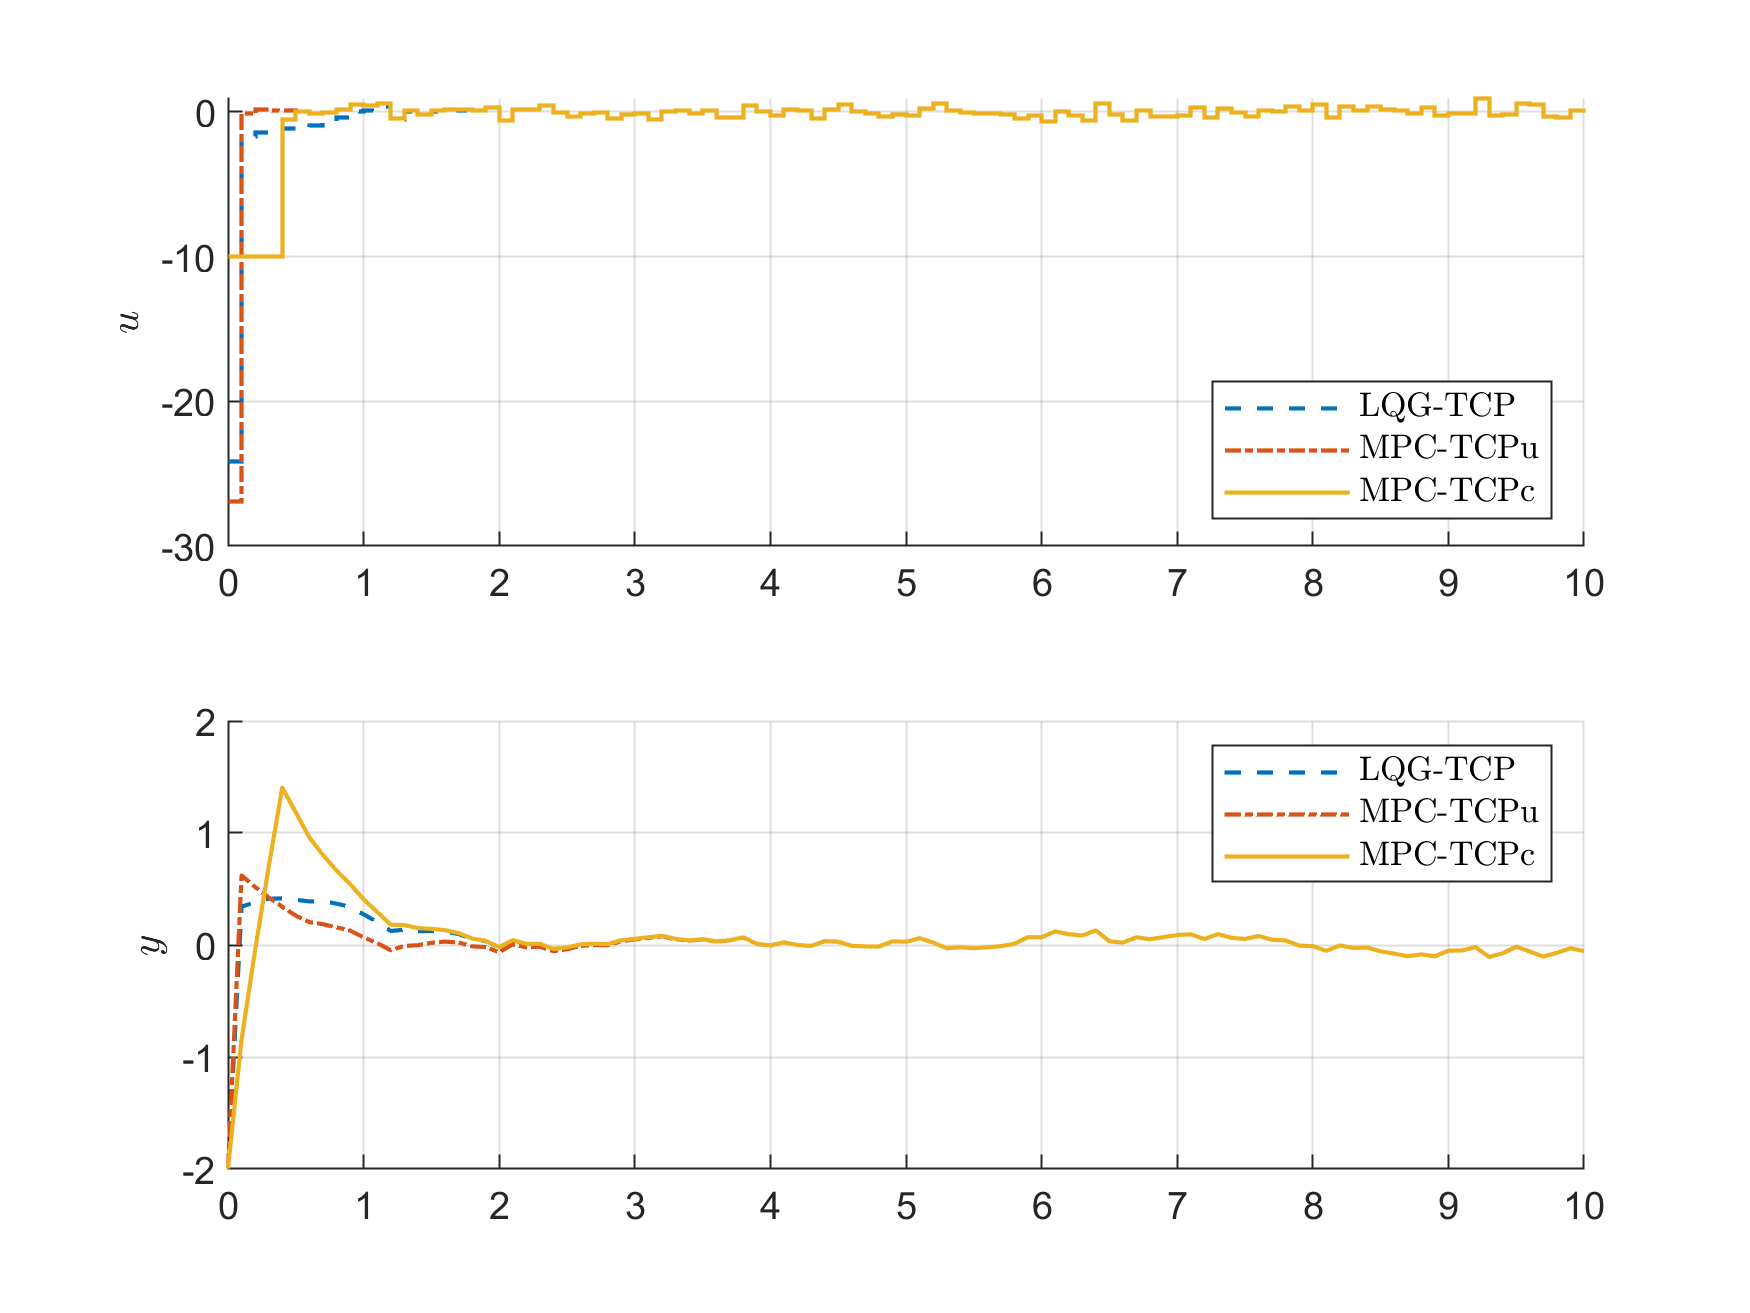
\includegraphics[width=1\linewidth]{figures/LQG_MPCu_MPCc_input+output}
		%	\caption{}
	%	\label{fig:}
	\end{figure}
\end{frame}

\begin{frame}{Ejemplo}
	\begin{figure}[!ht]
		\centering
		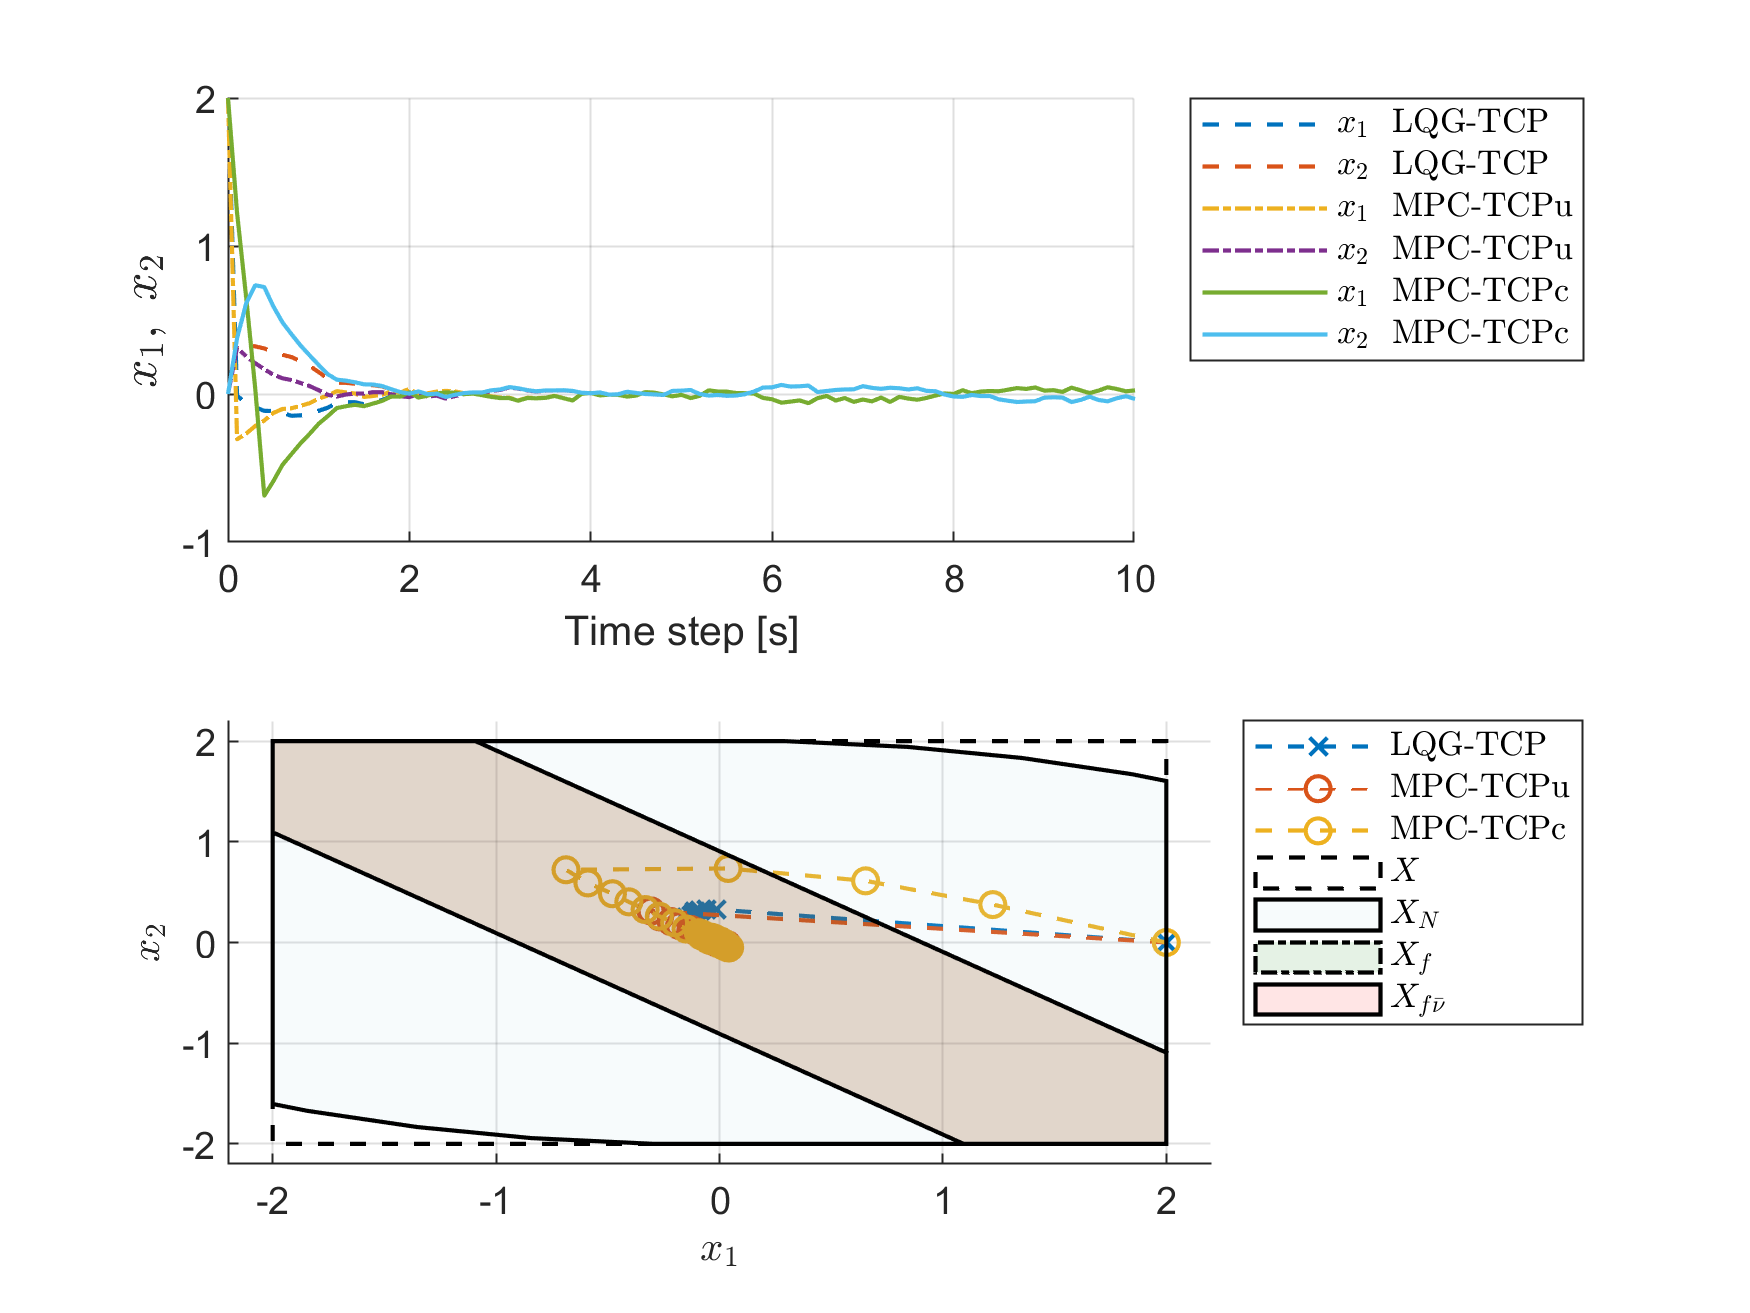
\includegraphics[width=1\linewidth]{figures/LQG_MPCu_MPCc_phaseplot}
		%	\caption{}
	%	\label{fig:}
	\end{figure}
\end{frame}

\begin{frame}[fragile]{Fin}
	20 años después... pero solo es la superficie.
	\Activate
	\begin{easylist}[itemize] \ListProperties(Space1=0cm,Space1*=0cm,Space2=0cm,Space2*=0cm)
		& MPC nolineal.
		& MPC explícito.
		& MPC robusto.
		& MPC estocástico.
		& MPC distribuido y descentralizado.
		& MPC adaptativo.
		& MHE (Moving Horizon Estimation)
		& ... 	
	\end{easylist}
	\Deactivate
\end{frame}



\section{Referencias}
\begin{frame}{Referencias}
%\renewcommand{\bibname}{REFERENCES}
\printbibliography
\end{frame}










\end{document}